

\subsection{signal details}
\label{sec:signaldetail}

For a complex signal transmission power, bitrate and attenuation of a Signal
can be mathematical mappings from space, frequency and time to double. So
we decided to store each of them by the ``Mapping``-interface which is able to
represent a mathematical mapping from an arbitary domain (time + $\mathbb{R}^n$)
to a double ($\mathbb{R}$) value.

\begin{figure}[H]
 \centering
 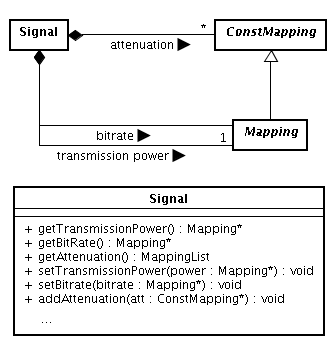
\includegraphics[width = 0.6\textwidth]{SignalDetail/signal_members.png}
 \caption{signal members (TX-power, bitrate and attenuation)}
 \label{fig:signal members detail}
\end{figure}

ConstMapping represents a mathematical mapping which can not be changed
arbitary, see section \ref{mapping detail} for details.

So transmission power, bitrate and attenuation are each seperate Mappings. To
get the filtered (attenuated) transmission power its Mapping is multiplied with
every attenuation Mapping.
\newpage

\subsubsection{Mapping overwiev}

Since Mappping has to be able to map from an arbitary domain (with arbitary
dimenensions) to a double value we need some structures to represent a
dimension, a domain and the arguments for a mapping in a specific domain.

This leads to the following structure.

\begin{figure}[H]
 \centering
 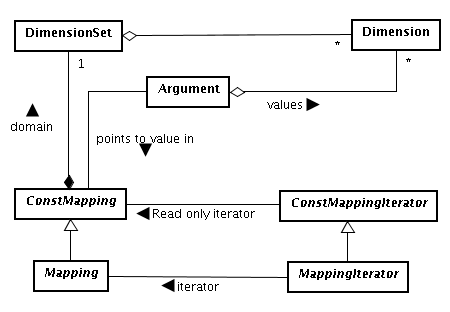
\includegraphics[width = 0.82\textwidth]{SignalDetail/mapping_detail.png}
 \caption{mapping details}
 \label{fig:mapping detail}
\end{figure}

\begin{figure}[H]
 \centering
 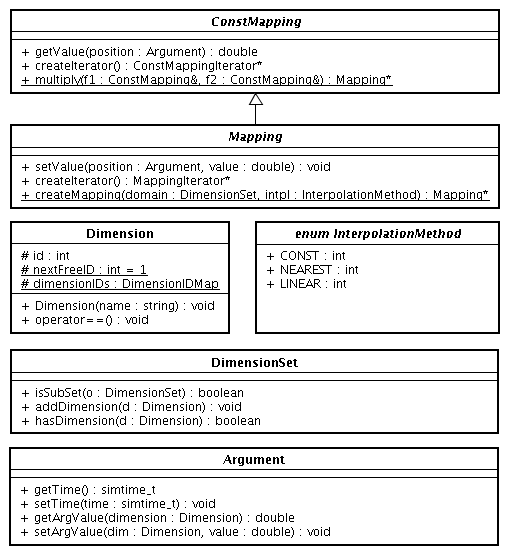
\includegraphics[width = 0.9\textwidth]{SignalDetail/mapping_members.png}
 \caption{mapping members}
 \label{fig:mapping members}
\end{figure}

Every instance of DimensionSet has at least the time as Dimension.
\newline

An instance of the Mapping interface has to provide random read and write access
per setValue() and getValue() method. This means if you call setValue() with an
valid Argument and the new value any following call of getValue() with the same
Argument has to return the new value.
\newline

%TODO: interpolation

Since the attenuation mappings does only need random read access but no write
access there is the ConstMapping-interface which basically is a Mapping without
the setValue()-method (or more precisely, Mapping is a ConstMapping with a
setValue()-method). This way we are able to implement ConstMappings which
represent a simple (probably parameterised) mathematical function like a sinus
curve.
\newline

The Mapping interface provides a multiply functions which is able to multiply
instances of Mappings with each other. This method is used by the decider to
get the attenuated transmission power.
\newline

To create an instance of a class which implements the Mapping interface one can
use the static createMapping()-method which creates a Mapping with the passed
DimensionSet as domain. If the DimensionSet parameter is ommited it creates an
Mapping with only time as domain. See section \ref{mapping detail} for details
on the returned Mapping implementation.

\subsubsection{iterating a Mapping}

The MappingIterator-interface provides an uniform way to iterate independent
from the underlying Mapping implementation.

\begin{figure}[H]
 \centering
 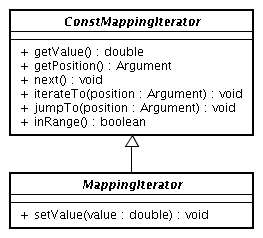
\includegraphics[width = 0.5\textwidth]
	{SignalDetail/mapping_iterator_member.png}
 \caption{mapping iterator details}
 \label{fig:mapping iterator detail}
\end{figure}

The next()-method iterates to the next position in the mapping, where this next
position actually is depends on the implementation of the Mapping. For
continous Mappings like the sinus curve this probably whouldn't be a particular
meaningful value. In fact this method is rather meant to be used for
implementations which use a number of key entries between which is interpolated.
But independent of the implementation of the underlying Mapping every iterator
has
to make sure that the Argument value of the position after the call of next is
compared greater than the Argument of the position before. This is possible
because Arguments can be sorted by the unique ids of their dimensions and the
the according values of the Argument.
\newline

While the jumpTo()-method is able to move the Iterator to an arbitary (but
valid) specified position the position passed to the iterateTo()-method has to
be greater or equal to the current position of the iterator. Furthermore the
iterateTo()-method assumes that the passed new position is near the current
position of the iterator, if this prerequirement is met iterateTo() is faster
than the jumpTo()-method.
\newline

Similar to ConstMapping the ConstMappingIterator is just a MappingIterator
whithout the setValue()-method.

\subsubsection{Mapping detail}
\label{mapping detail}

The type of the Mapping implementation returned by the createMapping()-method
of the Mapping interface depends on the passed DimensionSet parameter. If the
parameter is omitted or the DimensionSet defines only time as dimension the
returned Mapping is of type TimedMapping, otherwise it is of type
MultiDimMapping.

\subsubsection{TimedMapping}

The TimedMapping works only for Mappings with only time as domain. The mapping
is implemented by a std::map which takes the time as key. At every call of
setValue() the value is stored with the passed time as key in the map.
A call to getValue() returns the previously stored value in the map if
available, if no value is stored at this position it interpolates between the
nearest entries in the map to calculate the value at the queried position. 
\newline
%TODO: interpolation method

The MappingIterator for the TimedMapping makes use of the iterator of the
std::map. Since a MappingIterator has to be able to iterate to any
position inside the range of the domain of the Mapping but the map-iterator can
only point to actual values inside the map the MappingIterator also stores the
actual position together with the map-iterator. 

Here is a short description what the methods of the MappingIterator of a
TimedMapping do:

\begin{description}
 \item getValue() uses the map-iterator and the stored actual position
to calculate the actual value (per interpolation).
 \item next() simply increases the map-iterator by one to the next
entry in the map. 
 \item jumpTo() sets the map-iterator to the entry next to
the position passed as parameter and stores the passed position as actual
position.
 \item iterateTo() increases the map-iterator until it points to an entry
near the position passed as parameter and stores the passed position as actual
position.
\end{description}

\subsubsection{MultiDimMapping}

The MultiDimMapping is able to represent any Mapping with at least one
other Dimension besides the time as domain. The multiple dimensions are realized
by a map of Mappings. Every MultiDimMapping has a std::map from double to
pointers to Mapping (\verb std::map<double, \verb Mapping*> ).
So a simple two-dimensional Mapping (time and channel for example) whould be a
MultiDimMap which map stores for every channel a sub-mapping. Every
sub-mapping whould be of type TimedMapping and represent the gradient over time
for the according channel.

The following figure visualizes the general structure of a multi-dimensional
mapping with MultiDimMapping.

\begin{figure}[H]
 \centering
 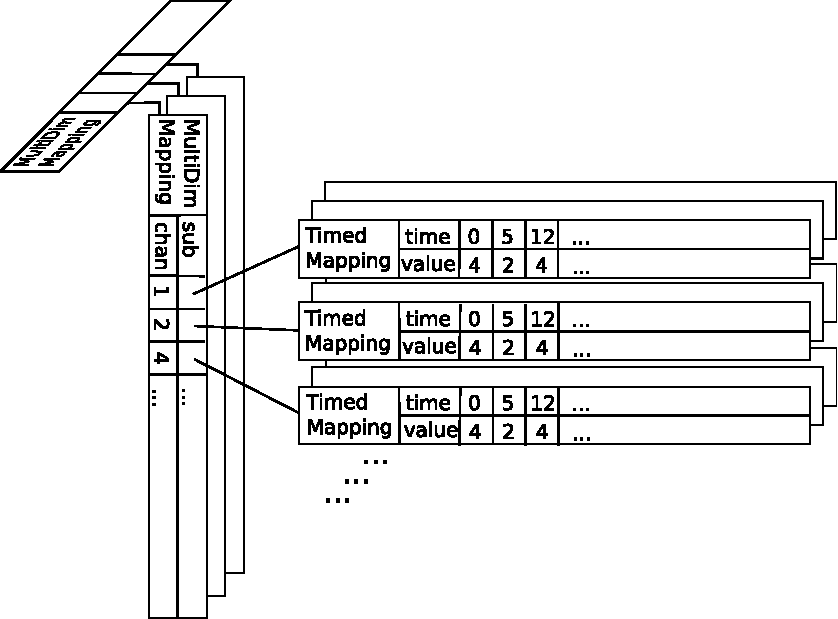
\includegraphics[width = 0.9\textwidth]{SignalDetail/mapping_scheme.pdf}
 \caption{multi dimensional signals}
 \label{fig:mappingscheme}
\end{figure}

So every dimension of the domain is represented by a layer of instances of
MultiDimMapping (respectively TimedMapping for the last dimension - which is
always the time).
The order of the layers is determined by the Dimensions and therefor is the
same for every MultiDimMapping instance.
\newline

Like the TimedMapping a MultiDimMapping can not store a value for every
possible position in the domain of the Mapping. Therefore a call to getValue()
whould determine the sub-Mappings near the position of the passed
Argument-parameter and pass the Argument-parameter to the getValue()-Methods of
the near sub-Mappings, then it interpolates between the returned values. Thus
getValue() is realized by recursive calls of getValue() and interpolation
between their return-values.
\newline 

Iteration is implemented the same way, meaning recursively. Like the
TimedMappingIterator the MultiDimMappingIterator stores the current position
(as a member of type Argument) together with a map-iterator pointing to the
entry inside the map of sub-Mappings near the current position.
Besides that it also stores an MappingIterator for the sub-Mapping at the
current position. This is necessary because the mapping has to be able to
iterate recursively over the sub-mappings.
\newline
%TODO:interpolation

Here is a short description what the methods of the MappingIterator of a
MultiDimMapping do:

\begin{description}
 \item getValue() calls recursively the getValue() method of the
MappingIterator of the sub-mapping at the current position.
 \item next() calls hasNext() at the MappingIterator of the
sub-mapping, if it returns true its next() method is called, otherwise the
map-iterator for the current sub-mapping is increased by one to the next
entry and a MappingIterator for the new position is created. Thereby it is
assured that the entries in the whole Mapping are iterated in the correct order.
\item jumpTo() and iterateTo() work more ore less like the methods for the
TimedMappingIterator.
\end{description}